\documentclass[tikz,border=2pt]{standalone}
\usepackage{amsmath,amssymb}
\usepackage{pgfplots}
\pgfplotsset{compat=1.18}

\begin{document}
% Convolution for two independent Exp(1) variables. For a fixed total t = 2 the integrand
% f_X(x) f_Y(2 - x) = e^{-2} is constant on (0, 2); its area 2e^{-2} is the value f_{X+Y}(2).
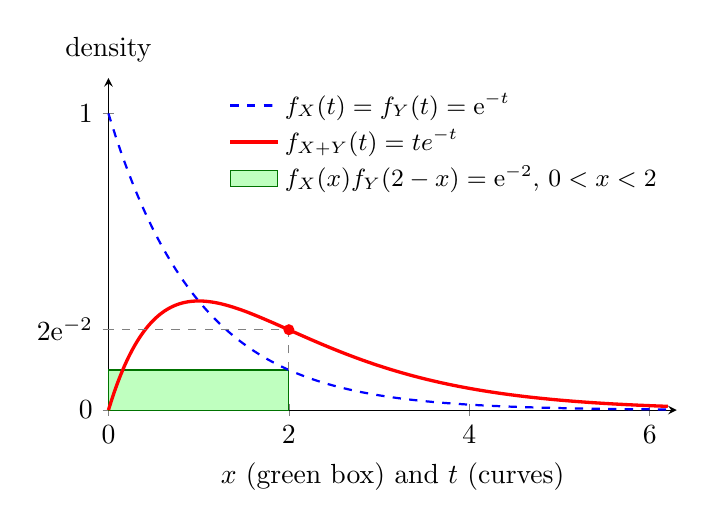
\begin{tikzpicture}
	\begin{axis}[
		axis lines=left, xmin=0, xmax=6.3, ymin=0, ymax=1.12,
		xtick={0,2,4,6}, ytick={0,0.271,1}, yticklabels={$0$,$2\mathrm{e}^{-2}$,$1$},
		xlabel={$x$ (green box) and $t$ (curves)}, ylabel={density}, ylabel style={rotate=-90, anchor=south, at={(axis description cs:0,1.02)}},
		samples=120, smooth, width=8.8cm, height=5.8cm, clip=false,
		legend style={draw=none, fill=none, font=\small, at={(0.99,0.99)}, anchor=north east}, legend cell align=left
		]
		\addplot[sharp plot, fill=green!25, draw=green!45!black, forget plot] coordinates {(0,0) (0,0.1353) (2,0.1353) (2,0)} -- cycle;
		\addplot[blue, thick, dashed, domain=0:6.2] {exp(-x)};
		\addlegendentry{$f_X(t)=f_Y(t)=\mathrm{e}^{-t}$}
		\addplot[red, very thick, domain=0:6.2] {x*exp(-x)};
		\addlegendentry{$f_{X+Y}(t)=te^{-t}$}
		\addlegendimage{area legend, fill=green!25, draw=green!45!black}
		\addlegendentry{$f_X(x)f_Y(2-x)=\mathrm{e}^{-2}$, $0<x<2$}
		\draw[gray, dashed] (axis cs:2,0.1353) -- (axis cs:2,0.271) -- (axis cs:0,0.271);
		\fill[red] (axis cs:2,0.271) circle (2pt);
	\end{axis}
	
\end{tikzpicture}
\end{document}
